\begin{myblock1}{\Large The EBRAINS Neuromorphic Computing Platform \phantom{\Huge $\beta$}}

    \begin{tikzpicture}[remember picture,overlay]
        \node[xshift=-560mm,yshift=265mm] at (current page.center) {
            \adjincludegraphics[trim={0 {.0\height} 0 {.0\height}}, clip, width=30mm, cfbox=black 0.0pt 0pt 0pt]{\imgpath/EBRAINS_circle_2.pdf}
        };
    \end{tikzpicture}

    \vskip13mm
    % \large
    \centering{
        \textbf{EBRAINS} Research Infrastructure offers access to two unique large-scale neuromorphic computing systems:
    }

    \vskip6mm
    \begin{columns}[t]
        \begin{column}{0.46\textwidth}
            \begin{flushright}
                \underline{\textbf{BrainScaleS} : the physical model machine}\\[1mm]
                \scriptsize{Location: Heidelberg (Germany)}
            \end{flushright}
            \vskip-8mm
            \begin{columns}[c]
                \begin{column}{0.50\textwidth}
                    \vskip+3mm
                    \begin{figure}[t]
                        \centering
                        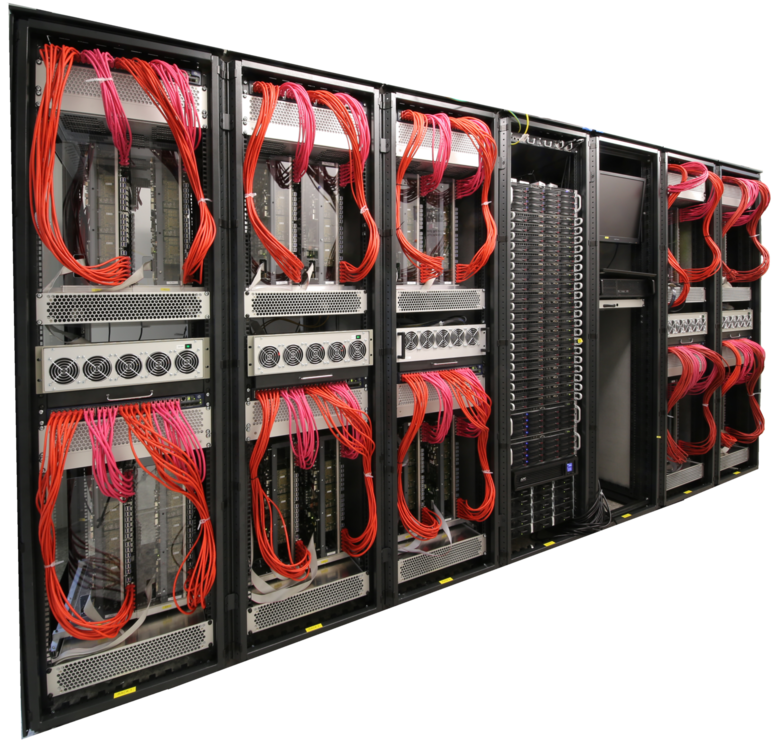
\includegraphics[width=1.0\textwidth,angle=00]{\imgpath/SP9_UHEI_RollUp_20160331_PlatformExported.png}
                    \end{figure}
                \end{column}
                \begin{column}{0.50\textwidth}
                    \begin{flushright}
                        \small{
                            20 wafer modules\\[2mm]

                            Local analogue computing\\
                            4 million neurons \\
                            1 billion plastic synapses\\[2mm]

                            Binary, asynchronous communication\\[2mm]

                            running at x10000 real-time
                        }
                    \end{flushright}
                \end{column}
            \end{columns}
        \end{column}
        % \begin{column}{0.001\textwidth}

        % \end{column}
        \begin{column}{0.46\textwidth}
            \begin{flushleft}
                \underline{\textbf{SpiNNaker} : the many-core machine}\\[1mm]
                \scriptsize{Location: Manchester (UK)}
            \end{flushleft}
            \vskip-9mm
            \begin{columns}[c]
                \begin{column}{0.40\textwidth}
                    \begin{flushleft}
                        \small{
                            over 1 million cores\\[2mm]

                            up to 1 billion neurons \\
                            up to 1 trillion synapses\\[2mm]

                            address-based, small packet, asynchronous communication\\[2mm]

                            real-time simulation
                        }
                    \end{flushleft}
                \end{column}
                \begin{column}{0.60\textwidth}
                    \vskip+3mm
                    \begin{figure}[t]
                        \centering
                        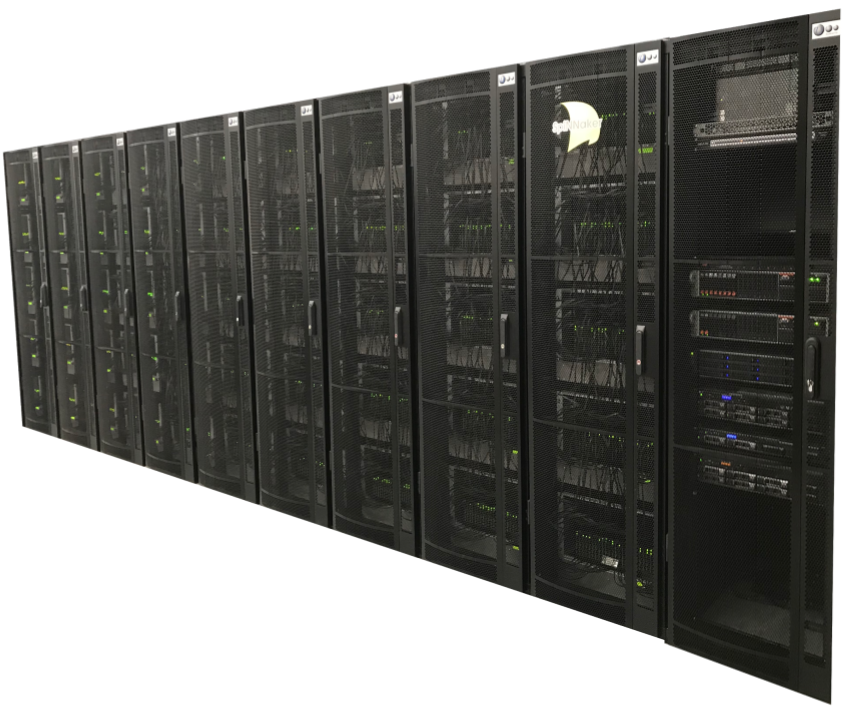
\includegraphics[width=.95\textwidth,angle=00]{\imgpath/SpNN_1Million.png}
                    \end{figure}
                \end{column}
            \end{columns}
        \end{column}
    \end{columns}
    \vskip-15mm
    \begin{columns}[t]
        \begin{column}{0.46\textwidth}
            \hspace{55mm} 
\includegraphics[height=27mm]{\imgpath/BrainScalesLogoNew}
        \end{column}
        % \begin{column}{0.03\textwidth}

        % \end{column}
        \begin{column}{0.46\textwidth}
            \hspace{80mm} 
\includegraphics[height=39mm]{\imgpath/SpiNNlogoHiResGIMP.png}
        \end{column}
    \end{columns}
\end{myblock1}